\section{Spring Framework}
Provides a programming and configuration model for modern Java-based enterprise applications - on any kind of deployment platform.

\subsection{Java Annotations}
\begin{itemize}
    \item Metadata that do not directly affect the code they annotate
    \item Uses
    \begin{itemize}
        \item Information for the compiler
        \item Compile-time and deployment-time proccessing
        \item Runtime processing
    \end{itemize}
\end{itemize}
\subsubsection{Examples}
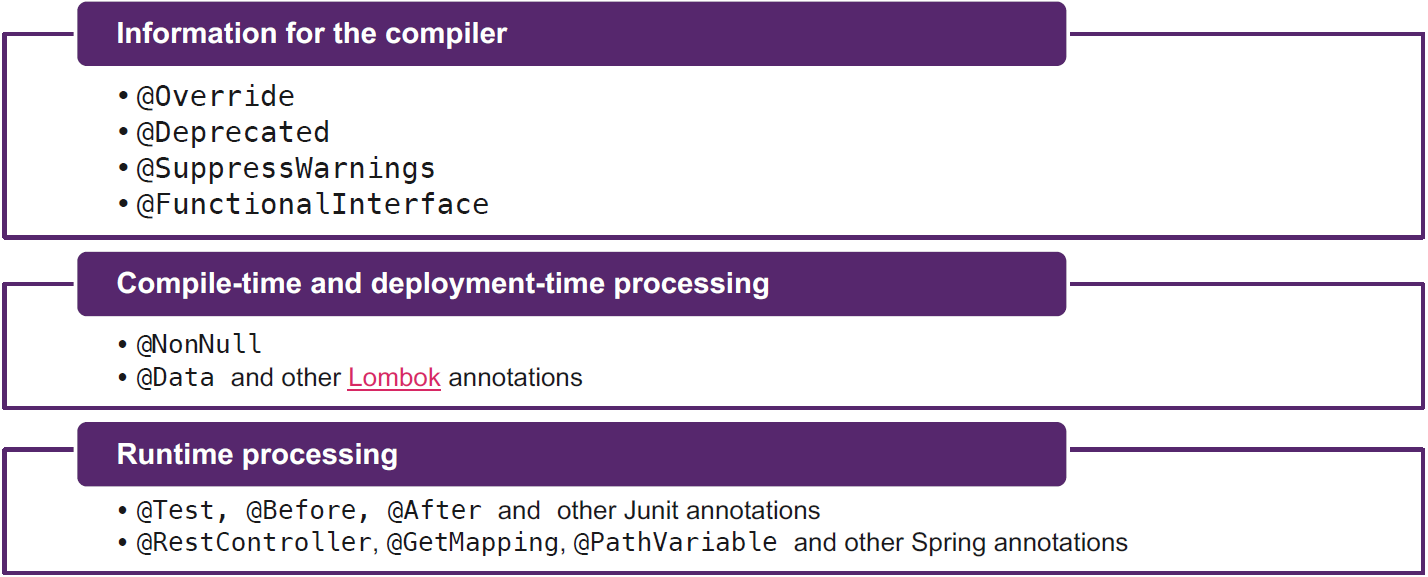
\includegraphics[width=\linewidth]{annotation.png}
\subsubsection{Declaring Annotations}
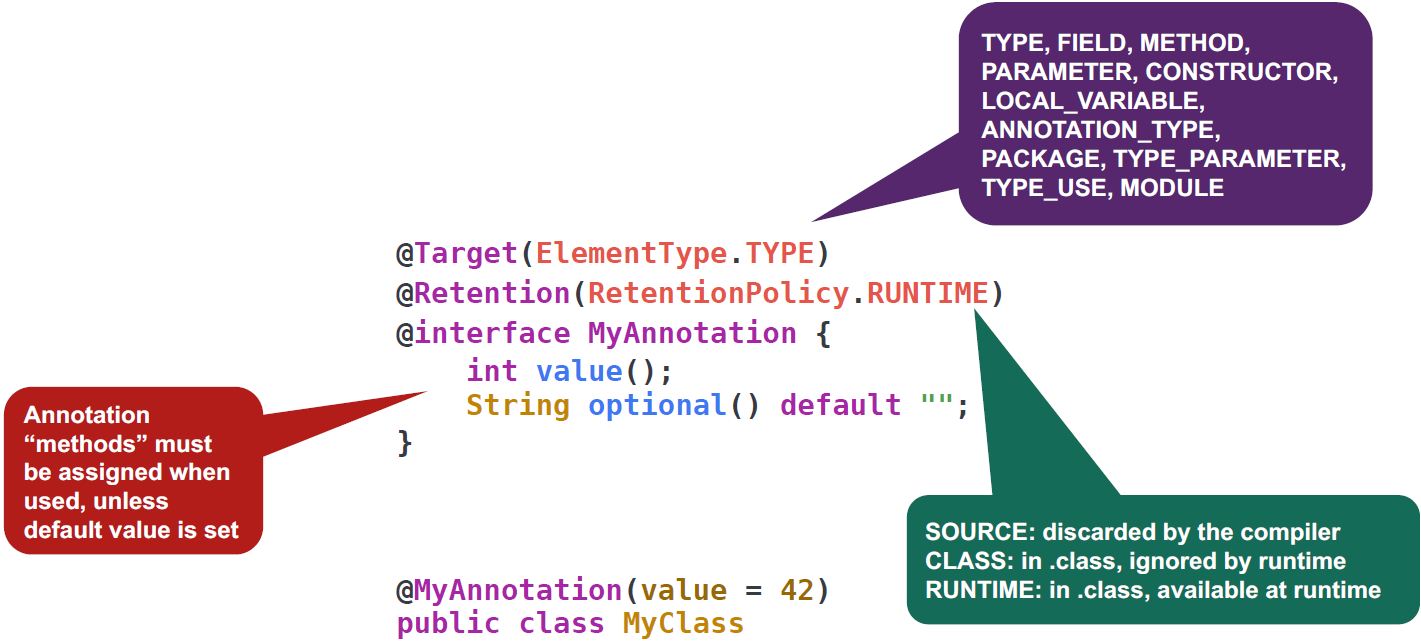
\includegraphics[width=\linewidth]{annotation_declaration.png}
\subsubsection{Processing Annotations}
\begin{itemize}
    \item Depending on retention policy
    \begin{itemize}
        \item processed by compiler
        \item during compilation by Annotation Processors
        \item at runtime using reflection
    \end{itemize}
    \item Processors need to be on the classpath to be recognized by the Java compiler
    \item Compiler then invokes the processor if it finds any annotations the processor has registerd
    \item Processors can generate new files, those can contain additional annotations
\end{itemize}

\subsection{Core Principles}
\begin{itemize}
    \item DI
    \item IoC
    \item Aspect Oriented Programming (AOP)
\end{itemize}

\subsection{Beans}
\begin{itemize}
    \item Form the backbone of the application
    \item Managed by the Spring IoC Container
\end{itemize}
\subsubsection{Scopes}
Control the lifetime of Beans
\begin{itemize}
    \item \textit{singleton}: (default) single object for each Spring IoC Container
    \item \textit{prototype}: Any number of instances
    \item \textit{request}: Lifecycle of a single HTTP request, each has its own instance
    \item \textit{session}: Lifecycle of a HTTP Session
    \item \textit{application}: Lifecycle of a ServletContext
    \item \textit{websocket}: Lifecycle of a WebSocket
\end{itemize}
\begin{lstlisting}
@Bean
@Scope('singleton')
public DataSource dataSource() { }
\end{lstlisting}

\subsubsection{Config Simplifications}
\textbf{@Component}: Spring creates beans automatically\\
\textbf{@ComponentScan}: Automatic scanning for components\\
\textbf{@Autowired}: Property is mapped to Constructor

\subsubsection{Aspect Oriented Programming (AOP)}
\begin{itemize}
    \item Mitigates cross-cutting concerns
\end{itemize}
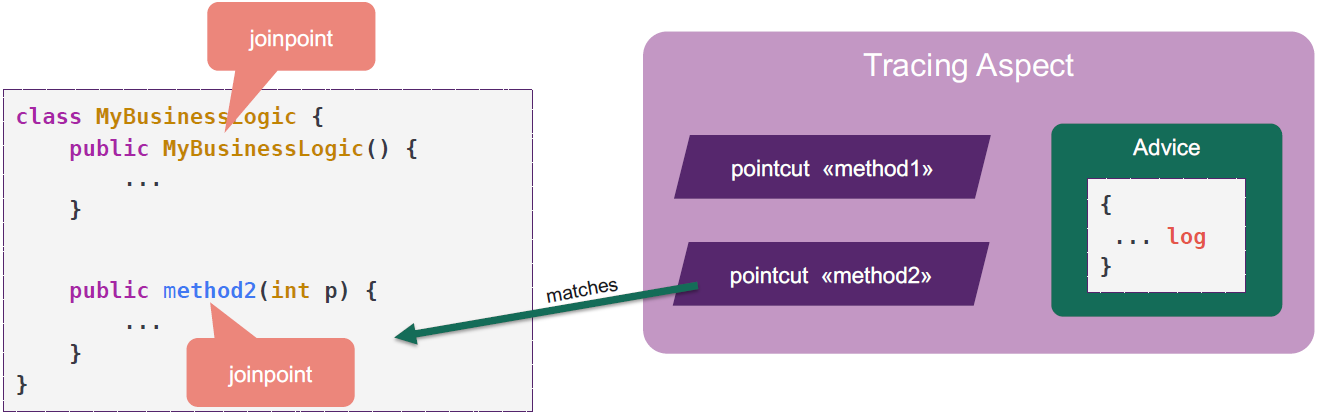
\includegraphics[width=\linewidth]{aop.png}
\begin{itemize}
    \item When a \textit{pointcut} pattern matches a \textit{joinpoint} being executed, an advice can be run
    \item Weaving is the compile or runtime technology to interleave the advice code into the joinpoints
\end{itemize}

\subsubsection{AspectJ}
\begin{itemize}
    \item Technology of Spring AOP
    \item Can be used on all objects
    \item Offers different approaches to weave aspects:
    \begin{itemize}
        \item Compile-time weaving (produces woven class files as output)
        \item Post-Compile weaving (weaves existing class files)
        \item Load-time weaving (binary weaving)
    \end{itemize}
\end{itemize}
